\documentclass{vgtc}

\ifpdf%                                % if we use pdflatex
  \pdfoutput=1\relax                   % create PDFs from pdfLaTeX
  \pdfcompresslevel=9                  % PDF Compression
  \pdfoptionpdfminorversion=7          % create PDF 1.7
  \ExecuteOptions{pdftex}
  \usepackage{graphicx}                % allow us to embed graphics files
  \DeclareGraphicsExtensions{.pdf,.png,.jpg,.jpeg} % for pdflatex we expect .pdf, .png, or .jpg files
\else%                                 % else we use pure latex
  \ExecuteOptions{dvips}
  \usepackage{graphicx}                % allow us to embed graphics files
  \DeclareGraphicsExtensions{.eps}     % for pure latex we expect eps files
\fi%

\graphicspath{{figures/}{pictures/}{images/}{./}} % where to search for the images

\usepackage{microtype}                 % use micro-typography (slightly more compact, better to read)
\PassOptionsToPackage{warn}{textcomp}  % to address font issues with \textrightarrow
\usepackage{textcomp}                  % use better special symbols
\usepackage{mathptmx}                  % use matching math font
\usepackage{times}                     % we use Times as the main font
\renewcommand*\ttdefault{txtt}         % a nicer typewriter font
\usepackage{cite}                      % needed to automatically sort the references
\usepackage{tabu}                      % only used for the table example
\usepackage{booktabs}                  % only used for the table example
\usepackage{tikz}
\usetikzlibrary{trees}
\usepackage{dot2texi}


%% If you are submitting a paper to a conference for review with a double
%% blind reviewing process, please replace the value ``0'' below with your
%% OnlineID. Otherwise, you may safely leave it at ``0''.
\onlineid{0}

%% declare the category of your paper, only shown in review mode
\vgtccategory{Research}

\title{Cauldron Chaos}

\author{Christoph Daxerer\thanks{e-mail: christoph.daxerer@chello.at}}
\affiliation{\scriptsize Software Engineering ba. VZ FH-Oberösterreich Hagenberg}

%% A teaser figure can be included as follows, but is not recommended since
%% the space is now taken up by a full width abstract.
%\teaser{
%  \includegraphics[width=1.5in]{sample.eps}
%  \caption{Lookit! Lookit!}
%}

%% Abstract section.
\abstract{
  For the V1\_VIREIL Virtual Reality course this paper describes the 
  design and impelemntation of a potion mixing game for the HTC Vive.
} % end of abstract


%%%%%%%%%%%%%%%%%%%%%%%%%%%%%%%%%%%%%%%%%%%%%%%%%%%%%%%%%%%%%%%%
%%%%%%%%%%%%%%%%%%%%%% START OF THE PAPER %%%%%%%%%%%%%%%%%%%%%%
%%%%%%%%%%%%%%%%%%%%%%%%%%%%%%%%%%%%%%%%%%%%%%%%%%%%%%%%%%%%%%%%%

\begin{document}

\firstsection{Introduction}

\maketitle

This paper 

\section{Design}

When designing a VR game it is crucial to understand the inherent nature of the medium. 
By addressing the strengths and weaknesses of VR already in the design phase, we can
avoid many of the pitfalls that plague VR games.

\subsection{Possibilities are Restrictions}

The HTC Vive features a vast set of interactions. Controllers, buttons, touchpads, all fully tracked. 
Although this is a great strength, it also means that the player has a lot of freedom. 

Often, freedom leads to confusion. To counteract this the decision was made not to limit the player,
but to engineer towards their intuition and expectations. Leading to the following design decisions:

\begin{itemize}
  \item \textbf{everything} the player expects to be interactable should be interactable
  \item controls should be intuitive and minimal
  \item the player should be able to move around freely
\end{itemize}

\subsection{Core Gameplay Loop}

The game is quite simple to learn. Throw ingredients into the cauldron in the correct order to create the 
desired potion. One player is the alchemist (in VR) and the other is the assistant (on the computer).

By navigating through a brewing graph the assistant can find out which ingredients are needed and 
in which order. The alchemist can then search for the ingredients in the room and throw them into the
cauldron.

\subsection{Ingredient System}

Every ingredient is made up of \emph{parts}. Each part has a \emph{material} and an \emph{amount}. Together they
make up the composition of the ingredient.

Materials follow a hierarchy. An example provides figure \ref{fig:MaterialHierarchyExample}.

\begin{figure}[ht]
  \centering
  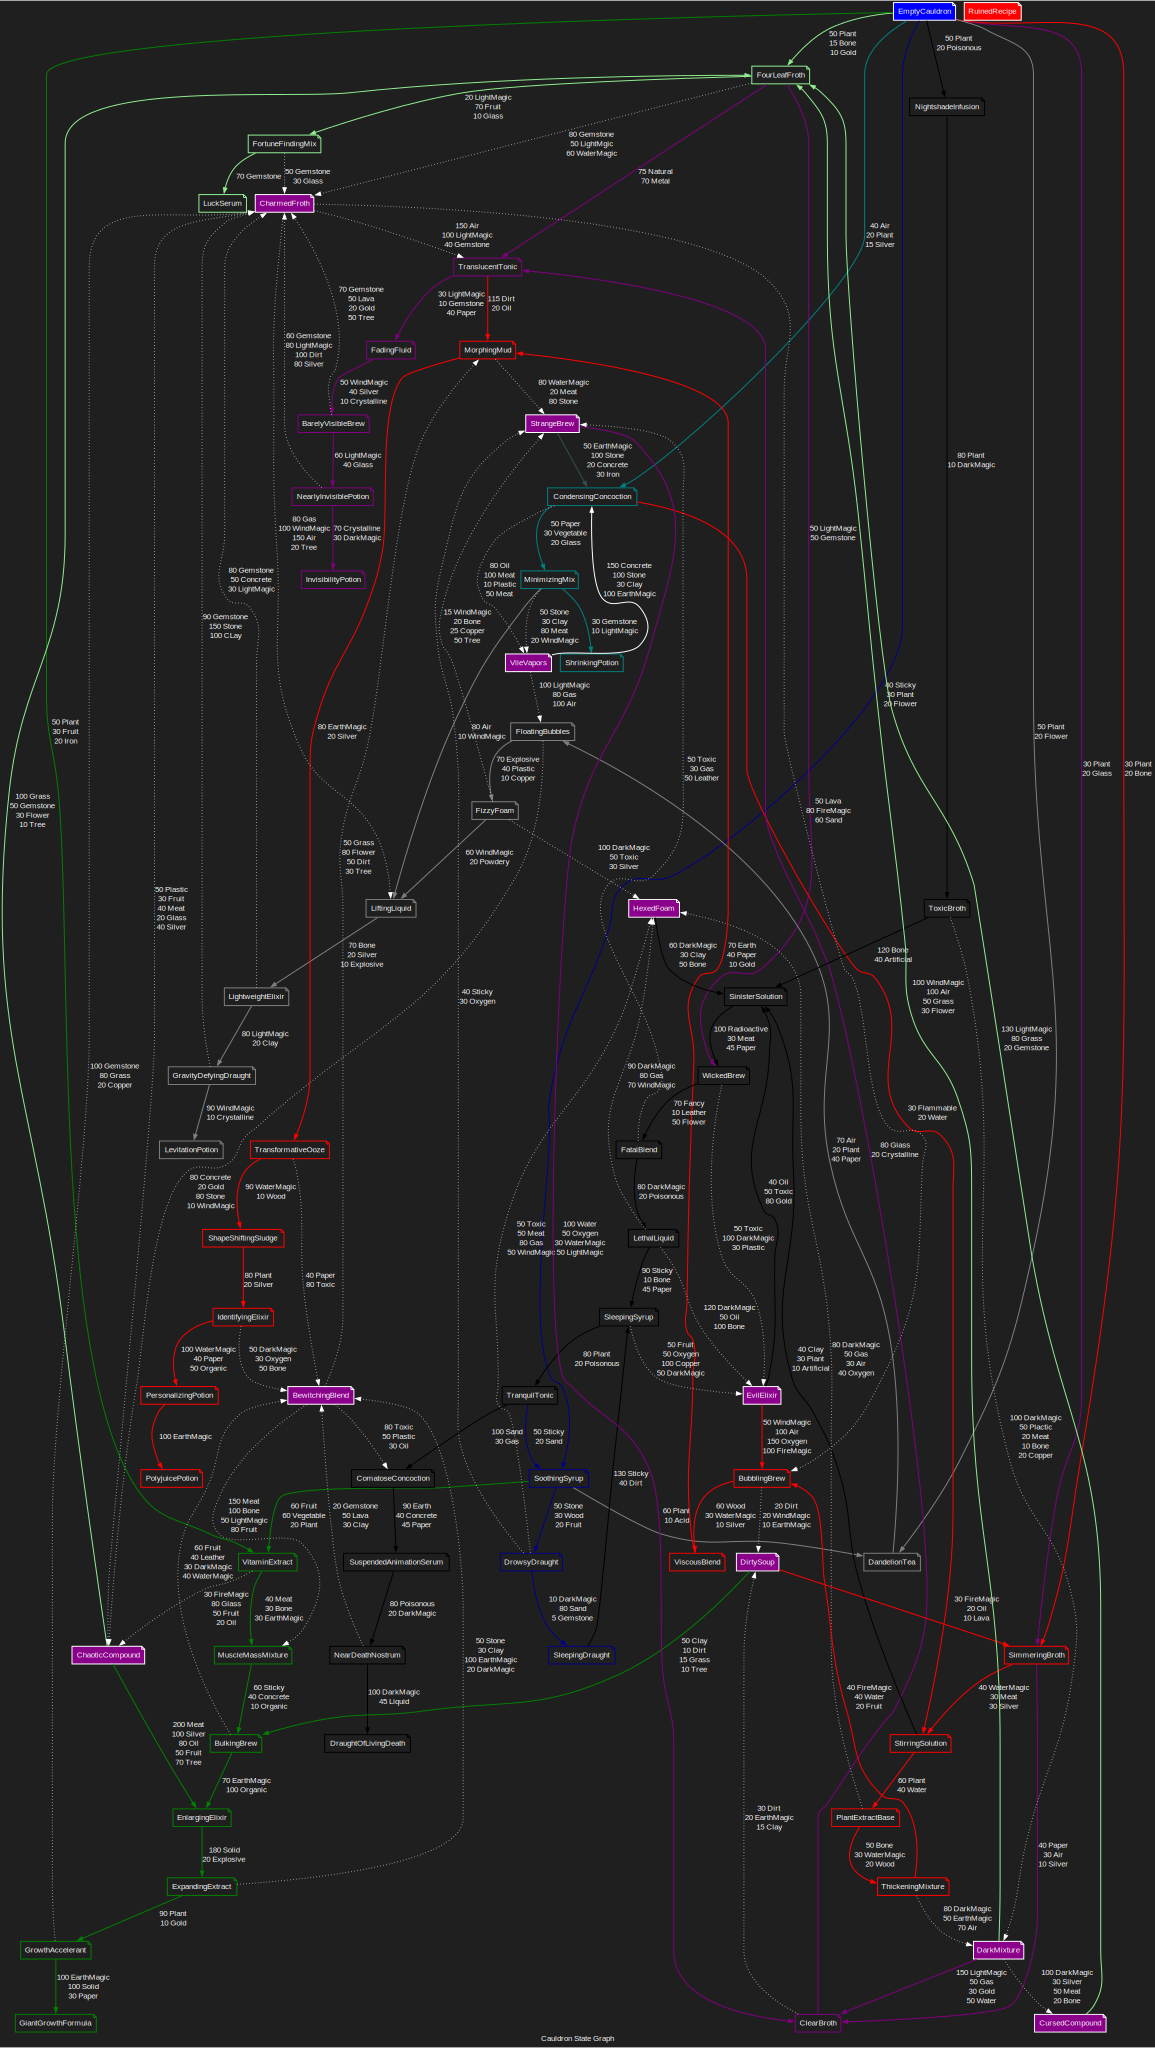
\includegraphics[width=0.45\textwidth]{pictures/test.png}
  \caption{An example of the material hierarchy.}
  \label{fig:MaterialHierarchyExample}
\end{figure}

\subsection{Engineering for Intuition}

\begin{figure}[ht]
  \centering
  \includegraphics[width=0.45\textwidth]{pictures/Screenshot_1.png}
  \caption{The initial view for the alchemist.}
  \label{fig:InitialView}
\end{figure}

The alchemist is immediately thrown into the game. Instinctively, the first thing they will do is
\textbf{orientate themselves}. This is why the game starts with the alchemist standing in the middle of the room as 
seen in figure \ref{fig:InitialView}.

After 5 seconds an \textbf{audible and visual cue} delivers the first task. After communicating with the assistant
a new problem promptly arises for the alchemist: "What are ingredients?".

Intuitively, the alchemist will try to pick up the first thing his brain classifies as "pick-up-able". Because
almost everything in the room is an ingredient this will work.

Having the object in his hand the alchemist will most likely either throw it into the cauldron or come to the next
problem: "How do I know what to throw into the cauldron?".

While working out what materials are needed, the alchemist needs to scout the house for ingredients. This is where
his curiosity will lead him to try and interact with the \textbf{Ingredient Inspect Station}.

\section{Implementation}

To keep track of the materials, states and transitions, 

\subsection{Dot Parser}

\subsection{Ingredient Materials}

\subsection{Cauldron State Graph}

\subsection{Ingredients}

\subsection{Cauldron Content Shader}

Shader Explanation

\subsection{Ingredient Inspect Station}

Speaker

\subsection{Audio System}

Pooling and stuff

\section{Stumbling Blocks}

\subsection{SteamVR Don't Destroy On Load}

\acknowledgments{
The author wishes to thank Schmidt Alexander, Schachinger Julian and Unterberger Bernhard for testing and 
providing valuable feedback.}

\end{document}